\section{Related work}

Many previous works have explored how to visualize volumetric data with lenses and distortion features to address occlusion issues. One major challenge is to maintain the data structures when visualizing the distorted information. To ensure a good visual quality, ray casting techniques are used to produce high-quality images. The computation time of these deformations in volume rendering remains an issue, and the produced images can hardly be generated in an interactive way. Other techniques can support interaction thanks to geometrical deformation or specific application domain deformations.
In our paper, we introduce a new technique which allies high-quality rendering and fast computation to support the interactive visualization of lens-based deformation of volumetric data.

According to the classification of view deformations by Carpendale et al.~\cite{595268}, our framework uses a nonlinear radial distortion through an interactive lens in order to remove occluding items and keep the global context while magnifying a partially occluded item. Within the large body of work and variations of lens techniques, we frame our contribution as follows:
\begin{itemize}
\item we introduced an interactive deforming lens based on GPU accelerated ray-casting. Our lens magnifies and pushes aside occluding objects located in front of the designated focal point with an interactive frame-rate,
\item we allow flexible and real-time interaction with the modification of the local point of view, the customized bent ray and the lens deformation parameterization. The inner part of the lens can be independently modified to provide a different perspective on the designated focal point. 
\end{itemize}

In this section, we introduce previous work categorized by occlusion management and lens deformations techniques in volume rendering. 


\subsection{Occlusion management}
As mentioned by Elmqvist and Tsigas~\cite{4483791}, many studies about occlusion management had been investigated. Multiple viewports, characterized by a view paradigm based on two or more separate views, can be used to see the scene under different perspectives~\cite{WangBaldonado:2000:GUM:345513.345271}. Virtual X-ray methods make targets visible by turning occluding surfaces invisible~\cite{Burns:2008:ACC:1457515.1409107} or semitransparent. Kruger et al.~\cite{4015450} introduced an interactive technique called ClearView, which enables the user to focus on particular areas in the data while preserving context information without visual clutter by using transparency. Correa and Ma~\cite{5416704} proposed visibility-driven transfer functions that maximize the visibility of the intervals of interest and provide high-quality images of volume data. However, it is still challenging to design a good transfer function, especially when the system has to deal with heterogeneous data. For instance, in baggage inspection, a dissimulation strategy is to hide a threat among objects with the same density. For direct volume rendering, in addition to removing voxels according to their density values and position, Rezk-Salama and Kolb~\cite{CGF:CGF979} also took into account the voxels' occurrence on the casted ray. Later, Hurter et al.~\cite{6787171} selected voxels in feature spaces, such as color or intensity distribution.
Li et al.~\cite{Li:2012:LVV:2425296.2425325} proposed a system for luggage visualization where any object is clearly distinguishable from its neighbors. They performed virtual unpacking for luggage visualization by visually moving any object away from its original location. This is a tool to manage occlusion, but destroying the context and the potential removal of important information inside the volume (positioning, connectivity).  In our previous work~\cite{7819413}, we have proposed an interactive visualization system that can support volumetric data exploration with direct manipulation of voxels. Little work has been done with a ray-casting approach for volume manipulation due to the computational costs involved. In order to better preserve the global context while addressing local obstruction problems,  We extend our previous system with a lens that pushes aside occluding objects thanks to rays deformation.  

\begin{figure*} 
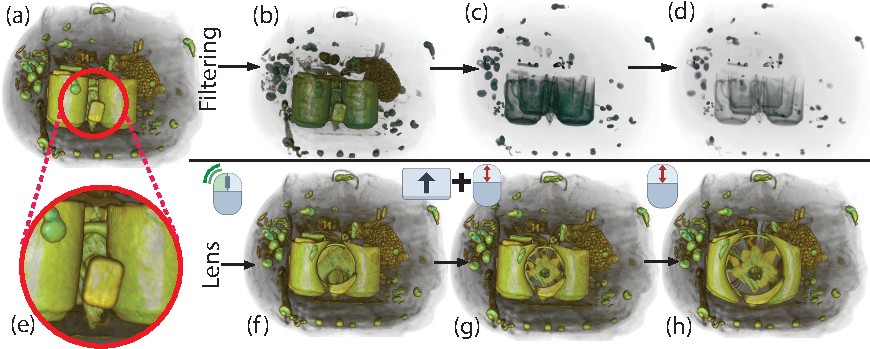
\includegraphics [width=\textwidth]{shuriken.pdf} 
\caption{  (a) A suspect object is spotted between a set of mugs. Almost all the densities are still displayed. (b)-(d)Filtering the densities using a classical 1D transfer function. (c) The materials with low densities are hidden. The object of interest is still visible. (d) The target disappears as we try to see through the mugs. (e) The user applies the lens tool on the targeted object (double-click). The animation starts with the opening of the lens. After half of the animation, the blunt object is magnified but only the area close to the location where the lens has been applied is visible. (f) The fish-eye field of view at the end of the animation allows perceiving all the front part of the shuriken. (g) The size of the lens is increased to magnify the shuriken (scroll). }
\label{f:baggage_lens}
\end{figure*}

\subsection{Lenses and deformations}
An interactive lens is a lightweight tool to solve a localized visualization problems by temporarily altering a selected part of the visual representation of the data~\cite{CGF:CGF12871}. Using this lens approach, we propose an interactive volume deformation based on GPU accelerated ray-casting to free a designated target from local occlusion while keeping the global context.

A lens is a parameterizable selection according to which a base visualization is altered. Typically, a lens is added to a visualization to interactively solve a specific localized problem. This property is very interesting with the aim of providing a focus+context solution to occlusion in volume rendering. Lenses can have different geometric properties not only defining their appearance, but also determining the selection, which is the subset of the data where these lenses take effect. The major geometric properties of a lens are shape, position, and size as well as the orientation.
The shape of a lens is usually chosen to fulfill the requirements of the application and is strongly linked to the lens function. Most virtual lenses are circular~\cite{1648236} or are rectangular~\cite{Kincaid:2010:SFA:1907651.1907963} as the real-world ones (magnifying glass, windows). Our lens has also a circular shape in order to remind its magnifying property. Some lenses, such as the  JellyLens~\cite{Pindat:2012:JCA:2380116.2380150} and the smart lenses~\cite{Thiede2008} can adapt their shape automatically according to the data. 
The position and the size parametrization can increase the flexibility of an interactive lens.
Modifying this position or size will set its focus on a different part of the data according to the user's interest. It is possible to update automatically these parameters in order to guide the user toward interesting events in the data~\cite{Tominski:2011:ECU:2336207.2336211}, or adjust the lens position according to predefined paths as the Routelens~\cite{Alvina:2014:RER:2598153.2598200} does. With this mind, our lens updates automatically its properties once a target has been selected. This allows a smooth transition towards an unobstructed and magnified area of interest. 

Lenses for volume visualization face challenges mainly related to spatial selection and occlusion. Wang et al. addressed these issues by proposing the Magic Lens~\cite{1532818}. This Magic Lens renders the obstructions with higher transparency and magnifies volumetric pre-computed features interactively or automatically in a pre-segmented dataset. In addition to interactively magnifying areas and objects of interest, our lens frees them from obstruction and allows local modification of the camera to see the target under other perspectives. Tong et al. proposed the GlyphLens~\cite{7539643} that removes the occluding glyphs by pulling the glyphs aside through the animation, but this tool is only well suited for systems where 3D volumetric dataset are visualized using glyphs. Lenses can create discontinuities between their inner part and the rest of the volume. Deformation can be a solution to this discontinuity issue.   

Hsu et al. developed a framework that can generate non-linear sampling rays that smoothly project objects in a scene at multiple levels of detail onto a single image~\cite{Hsu:2011:RFM:2070781.2024165}. Such a technique requires a lot of computational time to render a single image from features of interest at different scales.
  Bruckner and  Groller~\cite{4015467} proposed exploded view for volume data by partitioning the volume into several segments, while Correa et al. proposed a framework~\cite{Correa:2007:IDD:1313046.1313163} allowing the users to physically or actively manipulate the geometry of a data object. McGuffin et al.~\cite{1250400} performed deformations using peeling to see hidden parts of the data. However, these techniques have the disadvantage of removing potentially important surrounding contextual information while trying to solve the local occlusion. 
 
 
Deformations can reveal predefined features in the dataset by taking into account the precomputed segmentation. Tong et al. proposed a deforming Lens which moves streamlines to observe the inner part of streamline bundles~\cite{7332955}. Some studies performed deformations using surgical metaphors ~\cite{4069230,Correa:2006:FAV:1187627.1187827} to see hidden parts of the volume, but they do not offer tools for local manipulation of the point of view which allows perceiving a target under a different perspective while keeping the global context. 

